\documentclass{article}
\usepackage[margin=1in]{geometry}
\usepackage{tikz-cd}
\usepackage{amsmath}

\begin{document}

\section*{Correlation of Knowledge Transfer Behaviors in Bees and Managers}

\begin{tikzcd}[row sep=5cm, column sep=5cm, cells={nodes={font=\large}}]
\text{Bee Species} 
\arrow[r, "Selection of Flowers based on Knowledge", dashed] 
\arrow[d, "Discernment from vast stimuli"', bend right=15]
& \text{Flowers} \arrow[d, "Offering quality resources", bend left=15] \\
\text{Manager A} \arrow[r, "Selective advice seeking", dashdotted]
& \text{Manager B}
\end{tikzcd}



\vspace{1cm}

\textbf{Key:}
\begin{itemize}
    \item[\textbf{---}] Represents a direct knowledge flow or interaction.
    \item[\textbf{- - -}] Symbolizes the discernment process, sifting through vast information to find quality knowledge.
    \item[\textbf{- $\cdot$ -}] Indicates a pattern or method used to discern valuable knowledge.
\end{itemize}

\vspace{1cm}

\textbf{Shared Behaviors in Knowledge Transfer:}
\begin{itemize}
    \item Both bees and managers are inundated with information and stimuli.
    \item Both must discern valuable knowledge from this vast pool, emphasizing quality over quantity.
    \item Patterns and methods are employed to sift through and determine the most relevant and valuable pieces of knowledge.
\end{itemize}

\vspace{1cm}

\textbf{Excerpt from BRT research:} 
``Moreover, with the world standing on the brink of an information overload, BRT's implications for a transformative approach to organizational knowledge management become paramount, advocating for a shift from quantity to quality, from sheer accumulation to purposeful alignment.''

\vspace{1cm}

\textbf{Excerpt from Chittka, Lars. The Mind of a Bee:}
``Less appreciated are the mental efforts required along the way: in visiting 1,000 flowers, the bee has to work 1,000 floral “puzzle boxes” whose mechanics can be as complicated as operating a lock (figure 1.4), and no two flower species are quite alike in the mechanics that have to be learned to gain access to their contents. While flying through a flower meadow, the bee is constantly bombarded with stimuli (color patterns, scent mixtures, electric fields) from multiple flowers of several species per second, requiring the bee to pay attention only to the most relevant stimuli and to suppress the rest. Between visits to 1,000 flowers, the bee may have to reject 5,000 other flowers that either are unfamiliar or have been found to be poorly rewarding, or only rewarding at a different time of day.''


\begin{tikzcd}[row sep=2.5in, column sep=2.5in, cells={nodes={scale=0.7,align=center}}]
& \textbf{GFGs} \ar[ld, "Bees' Actions" description] \ar[rd, "Managers' Actions" description] & \\
\textbf{Bees} \ar[r, "Knowledge Transfer", bend right] & \textbf{Nash Equilibrium} \ar[l, "Dynamic Equilibrium" description, bend right] \ar[u, "Nested Hierarchies" description] \ar[r, "Dynamic Equilibrium" description, bend right] & \textbf{Managers} \ar[l, "Knowledge Transfer", bend right] \\
& \textbf{Gödel's Incompleteness} \ar[u, "Inherent Instability" description] & \\
\end{tikzcd}

% Key
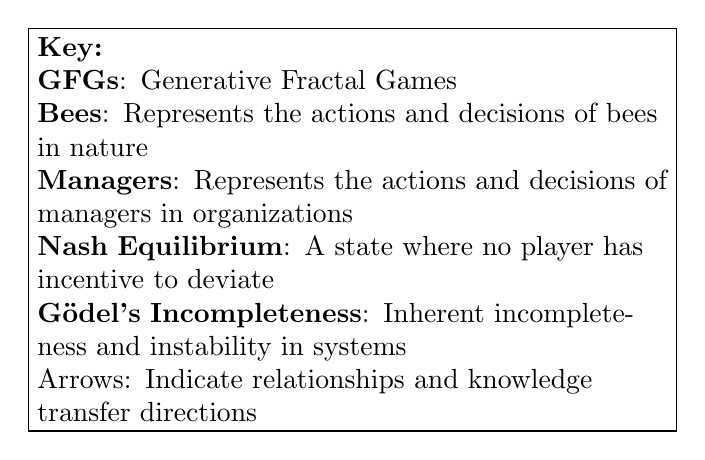
\begin{tikzpicture}
\node[draw, align=left, text width=8cm] at (0,0) {%
    \textbf{Key:}\\
    \textbf{GFGs}: Generative Fractal Games\\
    \textbf{Bees}: Represents the actions and decisions of bees in nature\\
    \textbf{Managers}: Represents the actions and decisions of managers in organizations\\
    \textbf{Nash Equilibrium}: A state where no player has incentive to deviate\\
    \textbf{Gödel's Incompleteness}: Inherent incompleteness and instability in systems\\
    Arrows: Indicate relationships and knowledge transfer directions};
\end{tikzpicture}

\begin{tikzcd}[cells={nodes={scale=0.5,align=center}}, row sep=2in, column sep=2in]
& \textbf{C. elegans Neural Network} \arrow[ld, "Small-world Properties" description] \arrow[rd, "Small-world Properties" description] & \\
\textbf{Bee-Pollination Network} \arrow[rr, "Similar Dynamics & Properties" description] && \textbf{Krackhardt Network}
\end{tikzcd}


\end{document}

